\documentclass[a4paper,12pt]{article}
\usepackage[utf8]{ inputenc}
\usepackage[ngerman]{babel}
\usepackage[a4paper, left=2.5cm, right=2.5cm]{geometry}
\usepackage{graphicx}
\usepackage{subcaption}
\usepackage{fancyhdr}
\usepackage{pdfpages}
\usepackage{listings}
\usepackage{hyperref}
\usepackage[official]{eurosym}
\usepackage{float}

\pagestyle{fancy}
\lstset{
	language=Matlab,
	breaklines=true,
	morekeywords={matlab2tikz},
	keywordstyle=\color{blue},
	morekeywords=[2]{1}, keywordstyle=[2]{\color{black}},
	identifierstyle=\color{black},
	stringstyle=\color{mylilas},
	commentstyle=\color{mygreen},
	showstringspaces=false,
	mathescape=true
	emph=[1]{for,end,break},emphstyle=[1]\color{red},
}

\lhead{Investitionsrechnung für Haushalte}
\chead{}
\rhead{Gruppe D}

\begin{document}
	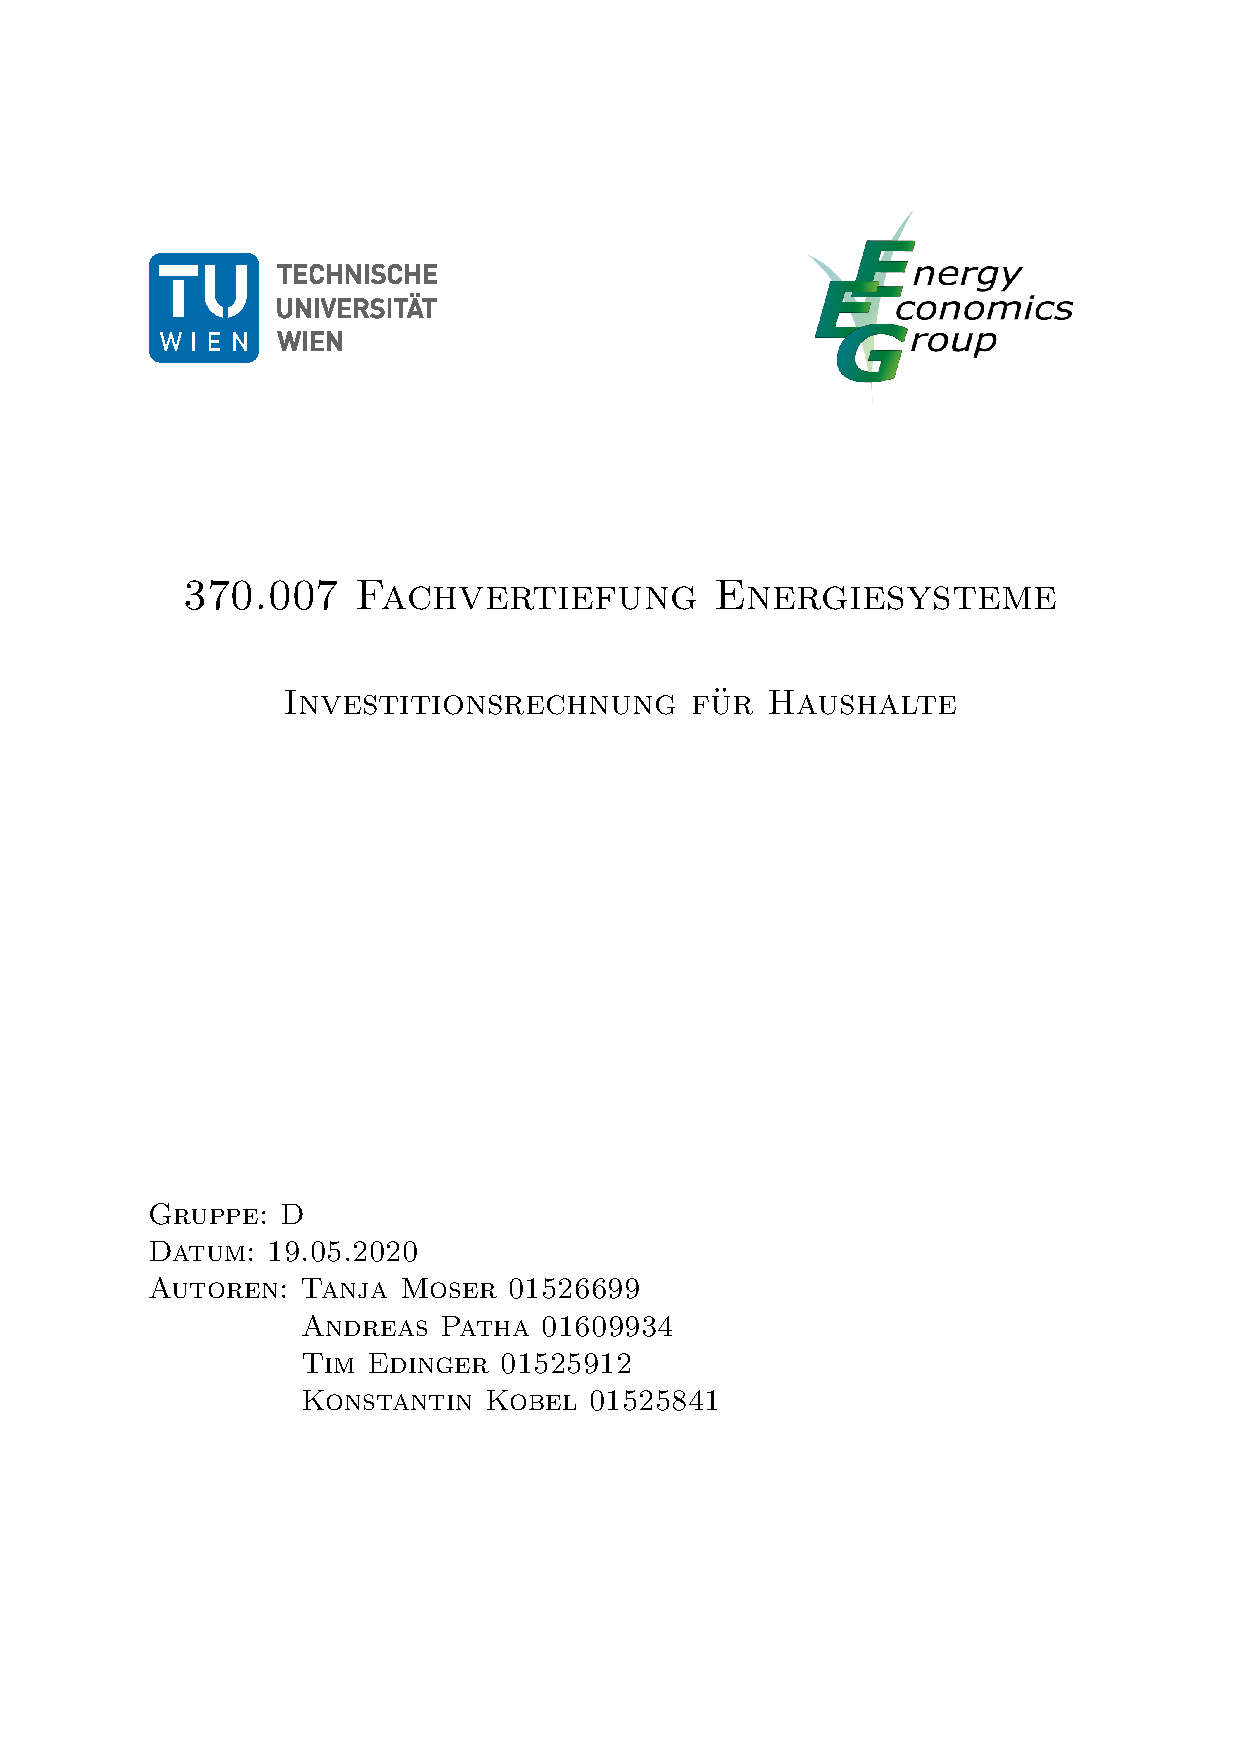
\includepdf{Protokoll_titlepage.pdf}

	\newpage
	\tableofcontents

	\newpage
	\section{Aufgabenstellung}
	\label{sec:Aufgabenstellung}
	Das Ziel der dritten Übung ist es, die Wirtschaftlichkeit einer PV-Anlage, für einen Haushalt, zu errechnen.\newline
	Die Wirtschaftlichkeitsrechnung ist ein wichtiges Instrument um Technologien aus volkswirtschaftlicher Sicht zu bewerten,
	Unternehmen eine Hilfe bei Investitionsentscheidungen zu bieten, staatliche Förderungen zu planen und Zahlungen an unterschiedlichen Zeitpunkten zu bewerten.
	\subsection{Aufgabe 3.1}
	\label{sec:Aufgabenstellung31}
	Aufgabe 3.1 befasst sich mit dem Barwert (= dem Kapitalwert) einer $10kWp$ PV-Anlage.\newline
	In dieser ersten Aufgabe wird davon ausgegangen, dass die gesamte Produktion verkauft wird.\\ \par
	\noindent Zur Berechnung werden folgende \textbf{Parameter} definiert:
	\begin{itemize}
		\item Der Zinssatz beträgt $4\%$.
		\item Die Systemkosten betragen $1200\mbox{\euro}/kWp$.
		\item Die Betriebskosten/die Versicherung belaufen sich auf $4\mbox{\euro}/(kWp\,a)$.
		\item Die Lebensdauer der PV-Anlage kann mit $25$ Jahren angenommen werden.
		\item Der $Einspeisetarif_{OeMAG}$ beträgt $8.24\,Cent/kWh$.
		\item Die $F\ddot{o}rderdauer_{OeMAG}$ beträgt $13$ Jahre.
		\item Die relevanten Spotpreise werden in der Datei $Spotpreise.mat$ zur Verfügung gestellt.
		\item Informationen zu Förderungen können folgendem Link entnommen werden:\newline
		\url{http://www.oem-ag.at/de/foerderung/photovoltaik/}
	\end{itemize}
	Es werden folgende \textbf{Annahmen} getroffen:
	\begin{itemize}
		\item Das Jahr 2016 steht exemplarisch für jedes kommende Jahr.
		\item Auch nach dem Vertragsende wird der Strom, bis zum Ende der Lebensdauer, am Spotmarkt verkauft. Die Preise entsprechen dabei den Preisen aus dem Jahr 2016.
	\end{itemize}
	Die \textbf{Aufgaben} lauten:
	\begin{itemize}
		\item[a)] Berechnen Sie den Barwert (= Kapitalwert) einer 10 kWp PV-Anlage unter der Annahme, dass die gesamte Produktion am Spotmarkt verkauft wird.
		\begin{itemize}
			\item Wie hoch dürfen die Investitionskosten maximal sein, damit die Wirtschaftlichkeit der Investition positiv bewertet wird (Barwert > 0)?
			\item Stellen Sie die Entwicklung des Kapitalwerts (=Barwert) der Investition über die Lebensdauer in einem Diagramm dar.
		\end{itemize}
		\item[b)] Führen Sie die Berechnung noch einmal unter der Annahme durch, dass Sie den aktuellen OeMAG Einspeisetarif für 13 Jahre erhalten.\newline Vergleich Sie diesen Fall mit dem nicht geförderten Fall.
	\end{itemize}
	\subsection{Aufgabe 3.2}
	In Aufgabe 3.2 wird der Eigenverbrauch der Haushalte berücksichtigt und nur noch der Überschuss der Produktion verkauft.\\ \par
	\noindent Folgende \textbf{Parameter} sind gegeben:
	\begin{itemize}
		\item Es handelt sich um eine $5kWp$ PV-Anlage.
		\item Das Einspeiseprofil der PV-Anlage wird in der Datei $PV_Einspeiseprofil.mat$ zur Verfügung gestellt.
		\item Der Standort der PV-Anlage ist Wien.
		\item Die Ausrichtung der PV-Anlage ist mit einem Azimut von $180^{\circ}$ und einem Neigungswinkel von $30^{\circ}$ gegeben.
		\item Die benötigte Leistung der Haushalte ist in der Datei $LeistungHaushalte.mat$ definiert.
	\end{itemize}
	Die \textbf{Aufgaben} lauten:
	\begin{itemize}
		\item[a)] Berechnen Sie den Eigenverbrauch und die Überschusseinspeisung einer $5kWp$-Anlage für 5 der gegebenen 30 Haushalte.
		\item[b)] Stellen Sie die Entwicklung des Eigenverbrauchsanteils und der Deckungsgrade der Haushalte für eine Anlagengröße von $0kWp$ bis $20kWp$ für die 5 Haushalte dar.
		\item[c)] Erstellen Sie eine Grafik, in der die Erzeugung, die Last und der Eigenverbrauch für die Woche 3 und 25 für Haushalt 1 dargestellt wird. Verwenden Sie für die Darstellung des Eigenverbrauchs die Plot-Funktion $area$.
	\end{itemize}
	\subsection{Aufgabe 3.3}
	In Aufgabe 3.3 sollen die Berechnungen von Aufgabe 3.2 erweitert werden.\\ \par
	\noindent Dazu werden folgende \textbf{Annahmen} getroffen:
	\begin{itemize}
		\item Für den Eigenverbrauch kann eine Ersparnis in Höhe des Haushaltsstrompreises angesetzt werden. Diese beträgt $15\,Cent/kWh$.
		\item Für die Überschusseinspeisung kann ein Einspeisetarif von $5\,Cent/kWh$ angenommen werden.
	\end{itemize}
	Die \textbf{Aufgaben} lauten:
	\begin{itemize}
		\item[a)] Erstellen Sie eine Investitionsrechnung (Barwert) für die 5 gegebenen Haushalte und einer Anlagengröße von $5kWp$. Vergleichen Sie dazu den Fall mit PV-Anlage mit dem Fall ohne PV-Erzeugung.
		\item[b)] Wie hoch dürfen die spezifischen Investitionskosten (EUR/kW) je Haushalt maximal sein, damit die Investition als wirtschaftlich gewertet wird?
	\end{itemize}
	\subsection{Aufgabe 3.4}
	In Aufgabe 3.4 soll eine Beurteilung von PV-Anlagen in Österreich, auf Basis der in den vorigen Aufgaben durchgeführten Berechnungen, getroffen werden.\\ \par
	\noindent Die \textbf{Fragen} lauten:
	\begin{itemize}
		\item[a)] Erstellen Sie eine Investitionsrechnung (Barwert) für die 5 gegebenen Haushalte und einer Anlagengröße von $5kWp$. Vergleichen Sie dazu den Fall mit PV-Anlage mit dem Fall ohne PV-Erzeugung.
		\item[b)] Wie hoch dürfen die spezifischen Investitionskosten (EUR/kW) je Haushalt maximal sein, damit die Investition als wirtschaftlich gewertet wird?
	\end{itemize}
	\newpage
	\section{Berechnungen}
	\label{sec:Berechnungen}
	\subsection{Zinsen}
	Wie bereits im Kapitel \hyperref[sec:Aufgabenstellung]{Aufgabenstellung} erwähnt, ist die Wirtschaftlichkeitsrechnung ein wichtiges Instrument für unterschiedlichste Akteure.\newline
	Einen starken Einfluss auf diese Berechnung haben Zinsen.\\ \par
	\noindent Zinsen bezeichnen in der Wirtschaft das Entgelt, das der Schuldner dem Gläubiger als Gegenleistung für vorübergehend überlassenes Kapital zahlt.\\ \par
	\noindent Sie haben mehrere Interpretationen und Funktionen:
	\begin{itemize}
		\item Funktion des \textbf{Entgelts für entliehenes Kapital}. In diesem Fall geht es um einen Mindest-Zinssatz der erreicht werden muss um die minimalen Kosten des Kapitaleinsatzes zu decken.
		\item Funktion der \textbf{Zeitpräferenz}. Sie beschreibt die Präferenz den Konsum in der Gegenwart zu tätigen und nicht auf einen zukünftigen Zeitpunkt zu warten.
		\item Funktion des \textbf{Allokationsmechanismus}. Diese Interpretation erlaubt Messungen und bietet eine Entscheidungshilfe. Die Funktion der Zinsen ist in diesem Fall, dass das "knappe Gut" Kapital möglichst sinnvoll verteilt wird.
		\item Funktion des \textbf{Risikoindikators}. Das mit der Investition verbundene Risiko hat einen starken Einfluss auf den Zinssatz.
	\end{itemize}
	Die Zahlungsströme (= Cash Flows) werden durch Zinsen gewichtet.
	\subsubsection{Aufzinsen}
	Beim Aufzinsen geht es um die Frage nach dem Wert von Kapital, nach $n$ Jahren. Für die Berechnung gehen wir davon aus, dass das Kapital zum Zeitpunkt $t=0$ eingezahlt wird.\\ \par
	\noindent Die Berechnung kann mit folgender Formel erfolgen:
	\begin{equation}
	K_n=K_0*(1+r)^n
	\end{equation}
	\begin{itemize}
		\item $K_n$ entspricht dem Wert des Kapitals nach $n$ Jahren.
		\item $K_0$ ist der Wert des Kapitals zum Zeitpunkt der Einzahlung. (zum Zeitpunkt $t=0$)
		\item $n$ ist die Dauer des Betrachtungszeitraums in Jahren.
		\item $r$ entspricht dem Zinssatz pro Jahr.
	\end{itemize}
	Der Wert des Kapitals wächst bei einem positiven Zinssatz $r$ nach $n$ Perioden exponentiell an.
	\subsubsection{Abzinsen}
	Bei der Bewertung einer Investition wird üblicherweise der Wert des zukünftigen Zahlungsstroms, zum Zeitpunkt $t=0$, ermittelt. Dieser Wert wird dann der Investition gegenübergestellt.\\ \par
	Die Berechnung kann mit Hilfe folgender Formel durchgeführt werden:
	\begin{equation}
	K_0=\frac{K_n}{(1+r)^n}
	\end{equation}
	\begin{itemize}
		\item $K_n$ ist der Wert des Kapitals nach $n$ Jahren.
		\item $K_0$ entspricht dem Wert des Kapitals zum Zeitpunkt der Einzahlung. (zum Zeitpunkt $t=0$)
		\item $n$ ist die Dauer des Betrachtungszeitraums in Jahren.
		\item $r$ entspricht dem Zinssatz pro Jahr.
	\end{itemize}
	\subsection{Barwertmethode}
	\label{sec:BerechnungenBarwertmethode}
	Die Barwertmethode ist eine Methode der dynamischen Wirtschaftlichkeitsberechnung bei der der Barwert (= Net Present Value $NPV$) errechnet wird. Sie liefert eine Aussage über die Sinnhaftigkeit einer Investition.\\ \par
	\noindent Zur Bestimmung des Barwertes einer Investition werden alle Zahlungsströme (= Cash Flows), eines bestimmten Betrachtungszeitraumes, auf den Zeitpunkt $t=0$, mit dem erwarteten Zinssatz $r$, abgezinst und addiert. Damit werden alle Zahlungen auf den Zeitpunkt $0$ bezogen.\\ \par
	\noindent Die Berechnung des Net Present Values erfolgt mit folgender Formel:
	\begin{equation}
	NPV=-I_0+\frac{E_1-A_1}{(1+r)}+\frac{E_2-A_2}{(1+r)^2}+...+\frac{E_n-A_n}{(1+r)^n}+\frac{L}{(1+r)^n}
	\end{equation}
	Andere Schreibweisen dieser Formel sind
	\begin{equation}
	NPV=-I_0+\frac{CF_1}{(1+r)}+\frac{CF_2}{(1+r)^2}+...+\frac{CF_n}{(1+r)^n}+\frac{L}{(1+r)^n}
	\end{equation}
	oder
	\begin{equation}
	NPV=-I_0+\sum_{i=1}^n\frac{CF_i}{(1+r)^i}+\frac{L}{(1+r)^n}
	\end{equation}
	\begin{itemize}
		\item $NPV$ entspricht dem Nettobarwert der Investition in Euro.
		\item $I_0$ sind die Investitionskosten zum Zeitpunkt $0$ in Euro.
		\item $E_i$ sind die Einnahmen in der Periode $i$ in Euro.
		\item $A_i$ sind die Ausgaben und Kosten in der Periode $i$ in Euro.
		\item $CF_i$ entspricht dem Cash Flow in der Periode $i$ in Euro. ($E_i-A_i$ entspricht einem Cash Flow)
		\item $r$ ist der gewählte Kalkulationszinssatz bei der Barwertrechnung bzw. der gesuchte Zinssatz bei der Berechnung des internen Zinsfuß.
		\item $L$ ist der Restwert der Investition am Ende des Betrachtungszeitraums in Euro.
		\item $n$ entspricht der Dauer des Betrachtungszeitraums in Jahren.
	\end{itemize}
	Wie bereits eingangs beschrieben, trifft die Barwertmethode eine Aussage über die Sinnhaftigkeit einer Investition.\newline Wenn der Wert $NPV$ größer als $0$ ist, lohnt sich die Investition. Ist der $NPV$ kleiner als $0$, sollte von einer Investition abgesehen werden.
	\subsection{Eigenverbrauch und Überschusseinspeisung}
	Bei den Berechnungen zum Eigenverbrauch und der Überschusseinspeisung wird von einem oder mehreren Haushalten, mit eigener Strom Produktion, ausgegangen.\\ \par
	In diesem Kontext sind drei Begriffe relevant:
	\begin{itemize}
		\item \textbf{Eigenverbrauchsanteil} - Der Eigenverbrauchsanteil entspricht dem Anteil des Eigenverbrauchs an der eigenen Gesamterzeugung.\\ \par
		\noindent Die Berechnung erfolgt über die Formel
		\begin{equation}
		Eigenverbrauchsanteil=\frac{Eigenverbrauch}{Gesamterzeugung}
		\end{equation}
		\item \textbf{Deckungsgrad} - Der Deckungsgrad ist das Verhältnis des Eigenverbrauchs zum gesamten Stromverbrauch.
		Er gibt den Anteil des Stromverbrauchs an, der durch die eigene Produktion gedeckt werden kann.\\ \par
		\noindent Die Formel, zur Berechnung, lautet
		\begin{equation}
		Deckungsgrad=\frac{Eigenverbrauch}{Stromverbrauch}
		\end{equation}
		\item \textbf{Energetischer Deckungsgrad} - Der energetische Deckungsgrad gibt das Verhältnis der Gesamterzeugung zum gesamten Stromverbrauch an.\\ \par
		\noindent Die Formel lautet
		\begin{equation}
		Deckungsgrad_{energetisch}=\frac{Gesamterzeugung}{Stromverbrauch}
		\end{equation}
	\end{itemize}
	\newpage
	\section{Ergebnisse}
	\subsection{Aufgabe 3.1}
	\subsubsection{3.1.a - Barwert einer 10kWp PV-Anlage}
	In Aufgabe 3.1.a soll der Barwert einer $10kWp$ Anlage berechnet werden. Die Parameter der PV-Anlage sind in Kapitel \hyperref[sec:Aufgabenstellung31]{Aufgabe 3.1} definiert.\newline
	Der Barwert der PV-Anlage wird mit der Formel aus Kapitel \hyperref[sec:BerechnungenBarwertmethode]{Barwertmethode} berechnet.\\ \par
	Der MATLAB Code, zur Berechnung des Barwerts, ist folgender:
	\begin{lstlisting}
	NPV = $-$Systemkosten*Anlagenleistung;
	for i = 1:25
		if i <= 9
			Preis_i = table2array(Spotpreis(:,i))./100;
		else
			Preis_i = table2array(Spotpreis(:,9))./100;
		end
		CF = sum(PV_profil.*10.*Preis_i)$-$Betriebskosten*Anlagenleistung;
		NPV = NPV + CF/(1+Zinssatz)^i;
	end
	\end{lstlisting}
	Daraus ergibt sich das in Abbildung 1 dargestellte Diagramm.\\ \par
	Die maximalen Investitionskosten für die positive Bewertung der Wirtschaftlichkeit, im Fall, dass die gesamte Produktion am Spotmarkt verkauft wird, sind $50.964\mbox{\euro}$.
	\begin{figure}[H]
		\centering
		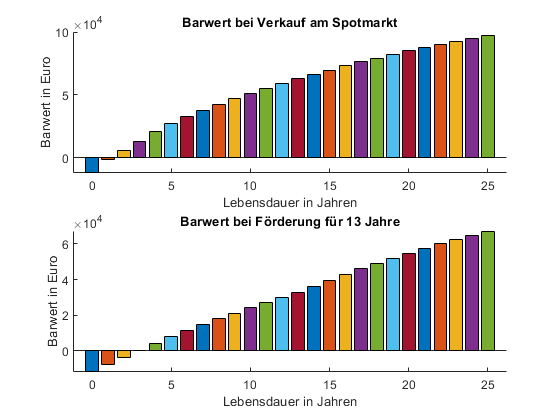
\includegraphics[width=12cm]{img/results/BarwertVergleich}
		\caption{TODO!}
	\end{figure}
	\subsection{Aufgabe 3.2}
	\subsection{Aufgabe 3.3}
	\subsection{Aufgabe 3.4}
	\newpage
	\section{Literatur}
	\begin{itemize}
		\item Literatur 1
	\end{itemize}
	\listoffigures
\end{document}